% 例 3：把 CD 平移到 AE，构成平行四边形 AECD
\documentclass[tikz,border=4pt]{standalone}
\usepackage{ctex}
\usepackage{amsmath}
\usetikzlibrary{calc, arrows.meta}
\begin{document}
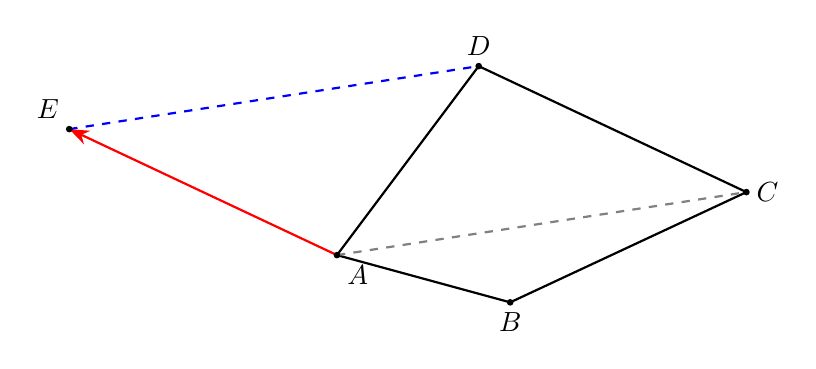
\begin{tikzpicture}[scale=1.0, thick]
  \coordinate (A) at (0,0);
  \coordinate (B) at (2.2,-0.6);
  \coordinate (C) at (5.2, 0.8);
  \coordinate (D) at (1.8, 2.4);
  % CD 向量 = D - C = (-3.4, 1.6)
  % AE 平行且等于 CD（同向），E = A + (D - C) = (-3.4, 1.6)
  \coordinate (E) at (-3.4, 1.6);

  \draw (A) -- (B) -- (C) -- (D) -- cycle;
  % 平移：AE 红实，CD 原黑色
  \draw[red, thick, -{Stealth[length=2.5mm]}] (A) -- (E);
  % 平行四边形 AECD：AE, ED, DC, CA
  \draw[blue, dashed] (E) -- (D);
  \draw[gray, dashed] (A) -- (C);

  \fill (A) circle (1.2pt); \fill (B) circle (1.2pt);
  \fill (C) circle (1.2pt); \fill (D) circle (1.2pt);
  \fill (E) circle (1.2pt);
  \node[below right] at (A) {$A$};
  \node[below] at (B) {$B$};
  \node[right] at (C) {$C$};
  \node[above] at (D) {$D$};
  \node[above left] at (E) {$E$};
\end{tikzpicture}
\end{document}
